% Provenance (never printed): old terminale S material on magmatism in
% subduction zones (volcanic arcs above the slab, water released by the slab
% and hydrous melting of the mantle wedge, andesitic volcanism and granitoid
% plutons, growth of the continental crust). Owner (Sync 0): volcanic arc,
% hydrous melting, granodiorite, batholith, continental growth. Subduction,
% slab, Wadati-Benioff zone, blueschist and eclogite are g11.06's; partial and
% decompression melting and peridotite g11.05's; andesite, diorite, rhyolite,
% pluton g11.08's; continental crust g12.01's; magma, explosive eruption Book 1's
% (g7): recalled, never redefined. Figures: figdata/grade-12/arc_magmatism.py
% (GVP volcanoes, ComCat NE Japan band, dry solidus via grade-11
% geotherm_solidus.py, wet solidus brackets of Wang 2020 and Kawamoto-Holloway 1997).
\chapter{Le magmatisme des zones de subduction}\label{ch:g12:subduction-magmatism}

Le 18 mai 1980, à 8~h~32 du matin, un séisme de magnitude 5.1 secoua le
mont Saint Helens. Aussitôt, le flanc nord du volcan, qui gonflait vers
l'extérieur d'environ deux mètres par jour, glissa d'un bloc~: la plus
grande avalanche de débris de l'histoire connue, environ \qty{2.5}{km^3} de
roches. Libéré de cette charge, le magma riche en gaz qu'il contenait jaillit
latéralement par la cicatrice, à pas moins de \qty{480}{km/h}, couchant les
forêts sur \qty{600}{km^2}. En quinze minutes, une colonne de cendres
s'éleva à plus de \qty{24}{km}, et l'éruption dura neuf heures.
Soixante et une personnes furent tuées ou ne furent jamais retrouvées.
% ledger: usgs:b2-msh-1980, usgs:msh-deaths

\begin{omfigure}
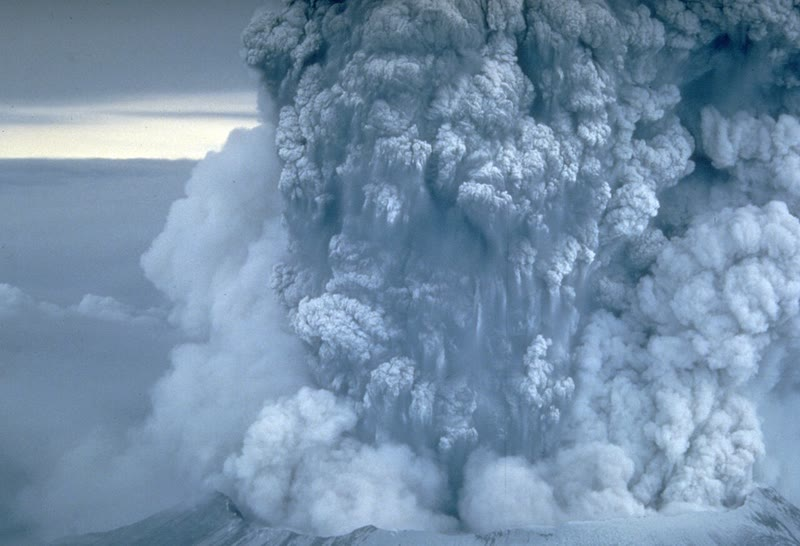
\includegraphics[width=0.55\linewidth]{images/book2/g12-swanson-st-helens-plume.jpg}

{\small La colonne de cendres du mont Saint Helens le 18 mai 1980, qui
s'éleva à plus de \qty{24}{km} en moins de quinze minutes. Photographie
Donald A.~Swanson, USGS (domaine public).}
\end{omfigure}
% ledger: photo:g12-st-helens, usgs:b2-msh-1980

Le mont Saint Helens fait partie d'une ligne de volcans --- Baker, Rainier,
Hood, Shasta et d'autres --- qui se dresse au-dessus de l'endroit où une
petite plaque océanique, la plaque Juan de Fuca, plonge sous l'Amérique du
Nord. Ce chapitre cherche pourquoi on trouve des volcans à cet endroit,
pourquoi leurs éruptions sont si souvent violentes, et ce que devient le
magma qui n'atteint jamais la surface.
% ledger: earle:cascades

\begin{recall}
Dans une \omterm{def:g11:subduction-zones:subduction}{zone de subduction}, une plaque de \omterm{def:g11:ocean-ridges:oceanic-lithosphere}{lithosphère océanique} replonge
dans le manteau sous une autre plaque~; ses séismes, la \omterm{def:g11:subduction-zones:benioff}{zone de
Wadati--Benioff}, suivent le \omterm{def:g11:subduction-zones:slab}{panneau plongeant} jusqu'à \qty{670}{km} de
profondeur (\cref{ch:g11:subduction-zones}). Le manteau est fait de
\omterm{def:g11:ocean-ridges:peridotite}{péridotite}~; il est solide, mais une roche qui remonte et se trouve moins
comprimée peut fondre en partie, par \omterm{def:g11:ocean-ridges:partial-melting}{fusion par décompression}, comme sous
une dorsale (\cref{ch:g11:ocean-ridges}). L'\omterm{def:g11:igneous-rocks:rock-names}{andésite} est une \omterm{def:g11:igneous-rocks:volcanic-plutonic}{roche
volcanique} \omterm{def:g11:igneous-rocks:felsic-mafic}{intermédiaire} entre le basalte et la \omterm{def:g11:igneous-rocks:rock-names}{rhyolite}, la \omterm{def:g11:igneous-rocks:rock-names}{diorite} son
équivalent \omterm{def:g11:igneous-rocks:volcanic-plutonic}{plutonique}, et un \omterm{def:g11:igneous-rocks:intrusion}{pluton} un grand corps de magma refroidi sous
terre (\cref{ch:g11:igneous-rocks}). La \omterm{def:g12:continental-crust:continental-crust}{croûte continentale} est épaisse et
légère, faite surtout de roches granitiques dans sa partie supérieure
(\cref{ch:g12:continental-crust}). Une éruption explosive pulvérise le magma
sous l'effet de ses propres gaz (livre~1, année~7).
\end{recall}
% ledger: tulane:magma-types, tulane:intrusions, rg14:crust

\section{Les arcs volcaniques}

La plupart des volcans actifs à terre ne sont pas répartis au hasard. Sur
les 1214 volcans entrés en éruption depuis la fin de la dernière glaciation
et recensés dans le catalogue du Global Volcanism Program, 838 --- plus de
deux sur trois --- se dressent au-dessus d'une \omterm{def:g11:subduction-zones:subduction}{zone de subduction}. Autour du
Pacifique, ils forment un anneau presque continu, souvent appelé la ceinture
de feu, et chacune de leurs lignes court parallèlement à une fosse, du côté
de la plaque qui ne plonge pas.
% values: n_volcanoes 1214, n_subduction 838, frac_subduction 0.690 (arc_magmatism.py)
% ledger: data:gvp, tulane:arc

\begin{omfigure}
\begin{tikzpicture}
\begin{axis}[ommap, width=\linewidth, xtick={-180,-90,...,180}, ytick={-60,0,60},
  legend style={font=\scriptsize, at={(0.5,-0.13)}, anchor=north, legend columns=3,
    /tikz/every even column/.append style={column sep=6pt}}]
\addplot[fill=omLithAlluv, draw=black!45, line width=0.2pt, forget plot] table {figdata/out/shared-geo-land.dat};
\addplot[black!70, line width=0.5pt, forget plot] table {figdata/out/shared-geo-school-subduction.dat};
\addplot[fill=black!70, draw=none, forget plot] table {figdata/out/shared-geo-school-teeth.dat};
% computed in figdata/grade-12/arc_magmatism.py; ledger: data:gvp, data:pb2002, data:ne-land
\addplot[only marks, mark=triangle*, mark size=1.1pt, black!40] table[x=lon, y=lat] {figdata/out/grade-12-arc_magmatism-world-other.dat};
\addplot[only marks, mark=triangle*, mark size=1.3pt, omThm] table[x=lon, y=lat] {figdata/out/grade-12-arc_magmatism-world-sub.dat};
\addlegendimage{black!70, line width=0.5pt}
\legend{{autres volcans}, {volcans au-dessus d'une zone de subduction}, {fosse}}
\end{axis}
\end{tikzpicture}

{\small Les volcans actifs depuis la fin de la dernière glaciation, en rouge
quand ils se dressent au-dessus d'une \omterm{def:g11:subduction-zones:subduction}{zone de subduction}, avec les fosses
(trait noir, triangles sur la plaque chevauchante). Données~: Smithsonian
Global Volcanism Program~; limites de plaques de Bird (2003)~; terres
émergées d'après Natural Earth.}
\end{omfigure}
% values: n_subduction 838 of 1214 (arc_magmatism.py)

\begin{definition}[Arc volcanique]\label{def:g12:subduction-magmatism:arc}
Un \emph{arc volcanique}\index{arc volcanique} est une ligne de volcans
située sur la plaque chevauchante d'une \omterm{def:g11:subduction-zones:subduction}{zone de subduction}, parallèle à la
fosse, au-dessus de l'endroit où le \omterm{def:g11:subduction-zones:slab}{panneau plongeant} a atteint une
profondeur d'une centaine de kilomètres. C'est un \emph{arc insulaire}
quand il s'élève du fond de la mer, comme au Japon ou en Indonésie, et un
arc continental quand il se dresse sur un continent, comme dans les Andes
ou les Cascades.
\end{definition}
% ledger: tulane:arc, earle:arc-water, earle:cascades, sa06:slab-depth

Le bord de l'arc le plus proche de la fosse s'appelle le \textbf{front
volcanique}~: du côté de la fosse, il n'y a plus aucun volcan. À quelle
profondeur se trouve le \omterm{def:g11:subduction-zones:slab}{panneau plongeant} sous ce front~?

\begin{proposition}[Le panneau plongeant sous le front volcanique]\label{prop:g12:subduction-magmatism:depth}
Si le \omterm{def:g11:subduction-zones:slab}{panneau plongeant} est un plan incliné d'un angle $\theta$ à partir de
la fosse, et si le front volcanique se trouve à une distance horizontale $d$
de la fosse, alors le toit du \omterm{def:g11:subduction-zones:slab}{panneau} se trouve sous le front à une
profondeur
\[
  H = d \tan\theta .
\]
\end{proposition}

\begin{proof}
Prenons une coupe verticale perpendiculaire à la fosse. Le \omterm{def:g11:subduction-zones:slab}{panneau
plongeant}, la surface et la verticale située sous le front forment un
triangle rectangle, dont l'angle droit est sous le front~: le côté le long
de la surface vaut $d$, le côté vertical $H$, et l'angle à la fosse vaut
$\theta$. Donc $\tan\theta = H/d$.
\end{proof}

Une compilation de 839 centres volcaniques le long de \qty{33000}{km}
d'arcs a mesuré $H$ sous chacun d'eux~: en moyenne sur des tronçons d'arc
de \qty{500}{km}, il va de 72 à \qty{173}{km}, avec une moyenne de
\qty{105}{km}. Les arcs situés au-dessus de \omterm{def:g11:subduction-zones:slab}{panneaux} raides sont proches de
leur fosse, ceux qui surmontent des \omterm{def:g11:subduction-zones:slab}{panneaux} peu inclinés en sont loin, mais
le \omterm{def:g11:subduction-zones:slab}{panneau plongeant} se trouve toujours à une centaine de kilomètres sous
eux.
% ledger: sa06:slab-depth

\begin{method}[Trouver le panneau plongeant sous un volcan]\label{met:g12:subduction-magmatism:slab}
\begin{enumerate}
  \item Prendre les séismes d'une bande étroite perpendiculaire à l'arc, et
        tracer leur profondeur en fonction de leur distance le long de la
        bande, à l'échelle vraie.
  \item Garder les séismes plus profonds qu'environ \qty{70}{km}~: les plus
        superficiels se produisent aussi dans la plaque chevauchante et sur
        la faille qui sépare les deux plaques.
  \item Tracer la droite des séismes profonds, ou lire leur profondeur, sous
        le front volcanique~: c'est la profondeur du \omterm{def:g11:subduction-zones:slab}{panneau} à cet endroit.
  \item Vérifier avec $H = d\tan\theta$, en mesurant $d$ à partir de la
        fosse et le pendage $\theta$ sur la coupe.
\end{enumerate}
\end{method}

\begin{omfigure}
\begin{tikzpicture}
\begin{axis}[omsection, name=jp, scale only axis, width=0.8\linewidth, height=0.2857\linewidth,
  xmin=0, xmax=700, ymin=0, ymax=250, y dir=reverse,
  xlabel={distance à l'est de \ang{138}~E (\unit{km})}, ylabel={profondeur (\unit{km})},
  xtick={0,100,...,700}, ytick={0,50,...,250}, tick label style={font=\small},
  every axis label/.append style={font=\small}]
% computed in figdata/grade-12/arc_magmatism.py; ledger: data:b2-usgs-ne-japan, data:gvp, data:pb2002
\addplot[only marks, mark=*, mark size=0.55pt, black!35] table[x=x_km, y=depth] {figdata/out/grade-12-arc_magmatism-jp-quakes.dat};
\addplot[omDef, line width=0.9pt, dashed] table[x=x_km, y=depth] {figdata/out/grade-12-arc_magmatism-jp-slab.dat};
\addplot[only marks, mark=triangle*, mark size=2.6pt, omThm] table[x=x_km, y expr=-7] {figdata/out/grade-12-arc_magmatism-jp-volc.dat};
\draw[omThm, densely dotted, line width=0.8pt] (axis cs:259.2,0) -- (axis cs:259.2,98.2);
\fill[omThm] (axis cs:259.2,98.2) circle (1.6pt);
\coordinate (front) at (axis cs:259.2,-14);
\coordinate (trench) at (axis cs:528.9,-14);
\coordinate (H) at (axis cs:262,60);
\coordinate (slab) at (axis cs:95,228);
\draw[black, line width=0.9pt] (axis cs:528.9,-12) -- (axis cs:528.9,0);
\end{axis}
\node[font=\scriptsize, anchor=south, text=omThm] at (front) {front volcanique (Iwate)};
\node[font=\scriptsize, anchor=south] at (trench) {fosse du Japon};
\node[font=\scriptsize, anchor=west, text=omThm, fill=white, inner sep=1pt] at (H) {\qty{98}{km}};
\node[font=\scriptsize, anchor=west, text=omDef, fill=white, inner sep=1pt] at (slab) {panneau plongeant, pendage d'environ \ang{20}};
\end{tikzpicture}

{\small Une coupe du nord-est du Japon à l'échelle vraie~: les séismes de
magnitude 4.5 ou plus entre \ang{37.5} et \ang{40.5}~N, de 1976 à 2025 (en
gris), les volcans de la même bande (triangles rouges) et la droite ajustée
sur les séismes plus profonds que \qty{70}{km} (en bleu, tirets). Deux sur
cinq des séismes superficiels situés à l'est de \ang{141.5}~E datent de
2011, l'année du grand séisme de mars. Données~: catalogue des séismes de
l'USGS~; Smithsonian Global Volcanism Program~; limites de plaques de Bird
(2003).}
\end{omfigure}
% values: shallow (<70 km) events east of 141.5 E: 3622, of which 1451 in 2011 (0.40); ledger usgs:tohoku
% values: jp_front_lon 141.0 (x 259.2 km), jp_trench_lon 144.12 (x 528.9), jp_front_trench_km 269.4, jp_dip_deg 19.98, jp_H_geom 98.0, bin_141_median 98.15, jp_slab_depth_front 105.6 (arc_magmatism.py)

\begin{example}[Le nord-est du Japon]\label{ex:g12:subduction-magmatism:japan}
Dans la bande de la figure, le volcan le plus oriental est l'Iwate, à
\ang{141.0}~E, et la fosse du Japon se trouve à \ang{144.1}~E. Un degré de
longitude y vaut $111.2\cos\ang{39} \approx \qty{86.4}{km}$, donc
$d \approx 3.12 \times 86.4
\approx \qty{270}{km}$. Les séismes profonds plongent d'environ \ang{20}, et
\[
  H = 270 \times \tan\ang{20} \approx \qty{98}{km}.
\]
Les séismes plus profonds que \qty{70}{km} situés sous le front lui-même
ont une profondeur médiane de \qty{98}{km}~: les deux valeurs concordent,
proches de la moyenne mondiale.
\end{example}
% values: km_per_deg_lon 86.415, jp_front_trench_km 269.4, jp_dip_deg 19.98, jp_H_geom 97.98, bin_141_median 98.15 (arc_magmatism.py)

\section{L'eau fait fondre le manteau}

Sous un arc, le \omterm{def:g11:subduction-zones:slab}{panneau plongeant} est froid, de même que la \omterm{def:g11:ocean-ridges:oceanic-lithosphere}{croûte
océanique} qui le surmonte~: elle ne peut pas fondre. Le magma doit venir du
manteau chaud situé au-dessus du \omterm{def:g11:subduction-zones:slab}{panneau}, le \textbf{coin de manteau}. Mais
ce coin ne remonte pas~: il ne peut donc pas fondre par décompression comme
sous une dorsale. Autre chose abaisse sa température de fusion~: l'eau.
% ledger: earle:settings (subducted crust stays cool), earle:flux-melting, earle:arc-water

La \omterm{def:g11:ocean-ridges:oceanic-lithosphere}{croûte océanique} est imprégnée d'eau de mer près de la dorsale où elle
se forme, et une grande partie de cette eau finit enfermée dans ses
minéraux, surtout dans la serpentine, issue de l'olivine et du pyroxène de
la croûte. À mesure que le \omterm{def:g11:subduction-zones:slab}{panneau} plonge et se réchauffe, ces minéraux se
décomposent et libèrent leur eau. L'eau monte dans la \omterm{def:g11:ocean-ridges:peridotite}{péridotite} chaude du
coin situé au-dessus.
% ledger: earle:arc-water, tulane:arc

\begin{definition}[Fusion hydratée]\label{def:g12:subduction-magmatism:hydrous-melting}
La \emph{fusion hydratée}\index{fusion hydratee@fusion hydratée} (ou fusion
par apport d'eau) est la \omterm{def:g11:ocean-ridges:partial-melting}{fusion partielle} d'une roche provoquée par un
apport d'eau, qui abaisse la température à laquelle la roche commence à
fondre.
\end{definition}
% ledger: earle:flux-melting, earle:arc-water

La température à laquelle une roche commence à fondre, à une pression
donnée, est son \textbf{solidus}. Pour la \omterm{def:g11:ocean-ridges:peridotite}{péridotite} sèche, il est bien
connu~; en présence d'eau, il est bien plus difficile à mesurer, et les
valeurs publiées diffèrent encore de 200 à \qty{600}{\celsius}. Les
expériences les plus récentes le placent entre 950 et \qty{1000}{\celsius}
à \qty{3}{GPa}, soit environ \qty{95}{km} de profondeur, et juste au-dessus
de \qty{1000}{\celsius} de 5 à \qty{11}{GPa}. La \omterm{def:g11:ocean-ridges:peridotite}{péridotite} sèche à
\qty{3}{GPa} ne commence à fondre que vers \qty{1470}{\celsius}~: l'eau
abaisse le solidus d'environ \qty{500}{\celsius}.
% values: dry_T_3gpa 1473.4, dry_minus_wet_3gpa 498, z_3gpa_km 95.2, dry_minus_wet_5gpa 658 (arc_magmatism.py)
% ledger: hirschmann:solidus, wang20:wet-solidus, kh97:wet-solidus, data:prem, earth:gmean

\begin{omfigure}
\begin{tikzpicture}
\begin{axis}[omrecord, name=sol, scale only axis, width=0.62\linewidth, height=6.2cm,
  xmin=700, xmax=1900, ymin=0, ymax=230, y dir=reverse,
  xlabel={température (\unit{\celsius})}, ylabel={profondeur (\unit{km})},
  xtick={800,1000,...,1800}, ytick={0,50,...,200}, axis y line*=left]
% computed in figdata/grade-12/arc_magmatism.py (dry: Hirschmann 2000 with PREM pressures; wet: Wang 2020, Kawamoto-Holloway 1997)
\addplot[omProp, line width=1.2pt] table[x=T_dry, y=depth_km] {figdata/out/grade-12-arc_magmatism-solidus.dat};
\addplot[omDef, line width=2.4pt] coordinates {(950,95.24) (1000,95.24)};
\addplot[omDef, line width=1.2pt] coordinates {(1000,155.6) (1000,216.3)};
\draw[-{Stealth}, black!70, line width=0.8pt] (axis cs:1460,95.24) -- (axis cs:1015,95.24);
\coordinate (gap) at (axis cs:1240,95.24);
\coordinate (dry) at (axis cs:1600,40);
\coordinate (wet) at (axis cs:1015,190);
\coordinate (wet3) at (axis cs:975,90);
\end{axis}
\begin{axis}[scale only axis, width=0.62\linewidth, height=6.2cm, at={(sol.south west)}, anchor=south west,
  xmin=700, xmax=1900, ymin=0, ymax=230, y dir=reverse, axis x line=none, axis y line*=right,
  axis line style={-}, ylabel={pression (\unit{GPa})},
  ytick={34.9,65.1,95.2,125.5,155.6,185.9,216.3}, yticklabels={1,2,3,4,5,6,7},
  every axis label/.append style={font=\small}, tick label style={font=\small}]
% pressure ticks at the PREM depths of 1-7 GPa (arc_magmatism.depth_at_pressure)
\end{axis}
\node[font=\scriptsize, anchor=south] at ([yshift=2pt]gap) {environ \qty{500}{\celsius}};
\node[font=\scriptsize, text=omProp, anchor=west, align=left] at (dry) {la péridotite sèche\\commence à fondre};
\node[font=\scriptsize, text=omDef, anchor=west, align=left] at (wet) {avec de l'eau~: juste\\au-dessus de \qty{1000}{\celsius}};
\node[font=\scriptsize, text=omDef, anchor=south] at ([yshift=2pt]wet3) {950--1000};
\end{tikzpicture}

{\small La température à laquelle la \omterm{def:g11:ocean-ridges:peridotite}{péridotite} du manteau commence à
fondre, en fonction de la profondeur~: à sec (en orange) et saturée en eau
(en bleu, les deux intervalles mesurés à ce jour). À la profondeur du
\omterm{def:g11:subduction-zones:slab}{panneau plongeant} sous les arcs, environ \qty{100}{km}, l'eau l'abaisse
d'environ \qty{500}{\celsius}. Sources~: Hirschmann (2000), avec les masses
volumiques de PREM~; Wang et ses collègues (2020)~; Kawamoto et Holloway
(1997).}
\end{omfigure}
% values: dry_T_3gpa 1473.4, dry_T_100km 1489.4, P_100km_gpa 3.157 (arc_magmatism.py)

L'eau fait donc ce que le seul chauffage ne pouvait pas faire~: elle fait
fondre une partie du coin chaud. Le magma, plus léger que le manteau solide
qui l'entoure, monte vers la surface~; une partie fait éruption, une part
bien plus grande reste et refroidit sous terre. L'endroit où l'eau est
libérée, et où le coin situé au-dessus est assez chaud pour fondre une fois
hydraté, est ce qui fixe le front volcanique à une centaine de kilomètres
au-dessus du \omterm{def:g11:subduction-zones:slab}{panneau}.
% ledger: earle:arc-water, tulane:arc, sa06:slab-depth, wang20:wet-solidus (position of the volcanic front controlled by melting in the wedge)

\begin{omfigure}
\begin{tikzpicture}[x=1cm, y=1cm, font=\scriptsize]
  % mantle
  \fill[omLithPeridotite!45] (0,-0.9) -- (7.4,-0.9) -- (7.5,-0.85) -- (6.5,-1.6) -- (5.5,-2.6) -- (4.5,-3.8)
    -- (4.25,-4.3) -- (0,-4.3) -- cycle;
  % sea and overriding continental crust
  \fill[omSea] (8.0,0) -- (12,0) -- (12,-0.4) -- (8.5,-0.4) -- cycle;
  \fill[omLithGranite!55] (0,0.1) -- (8.0,0.1) -- (8.5,-0.4) -- (7.5,-0.85) -- (7.4,-0.9) -- (0,-0.9) -- cycle;
  % the slab
  \fill[omLithBasalt!45, draw=black!60] (12,-0.4) -- (8.5,-0.4) -- (7.5,-0.85) -- (6.5,-1.6) -- (5.5,-2.6) -- (4.5,-3.8)
    -- (4.25,-4.3) -- (5.15,-4.3) -- (5.2,-4.3) -- (6.15,-3.15) -- (7.1,-2.2) -- (8.0,-1.55) -- (8.9,-1.2) -- (12,-1.2) -- cycle;
  \node at (10.4,-0.8) {lithosphère océanique};
  \node[anchor=west] at (6.0,-3.4) {panneau plongeant};
  % melting in the wedge, rising magma, plutons, volcano
  \fill[omThm!35, draw=omThm, densely dashed] (5.2,-1.75) ellipse (0.6 and 0.3);
  \node[omThm] at (5.2,-1.75) {fusion};
  \foreach \y in {-1.3,-1.05} \fill[omThm!80] (5.2,\y) circle (0.07);
  \fill[omLithGranite, draw=black!60] (4.75,-0.55) ellipse (0.42 and 0.2);
  \fill[omLithGranite, draw=black!60] (5.65,-0.4) ellipse (0.32 and 0.16);
  \node[anchor=east] at (4.25,-0.55) {plutons};
  \draw[omThm, line width=1pt] (5.2,0.1) -- (5.2,-0.85);
  \fill[black!65] (4.75,0.1) -- (5.2,0.75) -- (5.65,0.1) -- cycle;
  \node[anchor=south] at (5.2,0.8) {volcan};
  % water released by the slab
  \foreach \x/\y in {6.5/-1.6, 6.0/-2.1, 5.6/-2.5}
    \draw[omDef, -{Stealth}, line width=0.7pt, decorate, decoration={snake, amplitude=0.6pt, segment length=4pt, post length=1.5mm}]
      (\x,\y) -- ++(-0.3,0.3);
  \draw[omDef, line width=0.3pt] (7.5,-2.75) -- (6.35,-2.0);
  \node[omDef, anchor=west, align=left] at (7.5,-2.75) {eau libérée par\\le panneau plongeant};
  % labels and depth scale
  \node at (1.8,-0.4) {croûte continentale};
  \node[black!70, align=center] at (2.3,-3.6) {coin de manteau chaud\\(péridotite)};
  \node[anchor=south] at (8.5,0.12) {fosse};
  \draw[black!60, |-|] (0.4,0.1) -- node[left, align=right] {environ\\\qty{100}{km}} (0.4,-2.96);
  \draw[black!45, densely dotted] (0.4,-2.96) -- (5.2,-2.96);
  \fill[black!70] (5.2,-2.96) circle (1.3pt);
  \draw[black!45, densely dotted] (5.2,-2.96) -- (5.2,-2.05);
\end{tikzpicture}

{\small Le magmatisme d'une \omterm{def:g11:subduction-zones:subduction}{zone de subduction} (schéma sans échelle). En se
réchauffant, le \omterm{def:g11:subduction-zones:slab}{panneau plongeant} libère l'eau de ses minéraux~; elle monte
dans le coin de manteau chaud et le fait fondre en partie. Le magma
monte~: une partie fait éruption aux volcans, une part plus grande refroidit
dans la croûte sous forme de \omterm{def:g11:igneous-rocks:intrusion}{plutons}.}
\end{omfigure}
% ledger: earle:arc-water, earle:flux-melting, tulane:arc, tulane:ridge-rocks, sa06:slab-depth

\section{Andésites et granodiorites}

Les premiers liquides issus de la \omterm{def:g11:ocean-ridges:peridotite}{péridotite} hydratée ne sont pas
basaltiques. Dans les expériences à \qty{1}{GPa}, une \omterm{def:g11:ocean-ridges:peridotite}{péridotite} saturée en
eau donne des liquides de composition andésitique. En traversant la croûte
épaisse de l'arc, les magmas changent aussi en refroidissant, de
basaltiques à andésitiques et rhyolitiques. Les magmas d'arc sont donc plus
riches en silice que les basaltes des dorsales --- un magma andésitique en
contient de 55 à \qty{65}{\percent} ---, et ils transportent l'eau qui les
a produits.
% ledger: kh97:wet-solidus (andesitic melts at 1 GPa), tulane:eruptions, tulane:ridge-rocks, tulane:magma-types

Ces deux propriétés rendent leurs éruptions violentes. Plus un magma est
riche en silice, plus il est visqueux, et plus son gaz a de mal à
s'échapper~; une forte teneur en gaz et une forte viscosité, comme dans les
magmas andésitiques et rhyolitiques, favorisent les éruptions explosives.
Presque tous les stratovolcans se dressent au-dessus de \omterm{def:g11:subduction-zones:subduction}{zones de
subduction}~: des cônes hauts de milliers de mètres et larges de jusqu'à
\qty{20}{km}, aux pentes de 10 à 30 degrés, dont les éruptions vont de
coulées de lave calmes à des explosions. Sous le mont Saint Helens, une
chambre magmatique large d'environ \qty{1}{km} s'étend d'environ 6 à
\qty{14}{km} de profondeur.
% ledger: tulane:magma-types, tulane:eruptions, earle:composite

La plus grande partie du magma d'arc ne fait jamais éruption. Elle refroidit
lentement dans la croûte et cristallise en roches à gros grains.

\begin{definition}[Granodiorite]\label{def:g12:subduction-magmatism:granodiorite}
La \emph{granodiorite}\index{granodiorite} est une \omterm{def:g11:igneous-rocks:volcanic-plutonic}{roche plutonique} à gros
grains semblable au granite, mais qui contient plus de plagioclase que de
feldspath potassique~: de 20 à \qty{60}{\percent} de ses minéraux clairs
sont du quartz, et de 65 à \qty{90}{\percent} de son feldspath est du
plagioclase~; elle contient souvent de la biotite ou de la hornblende.
\end{definition}
% ledger: bgs:granodiorite

\begin{omfigure}
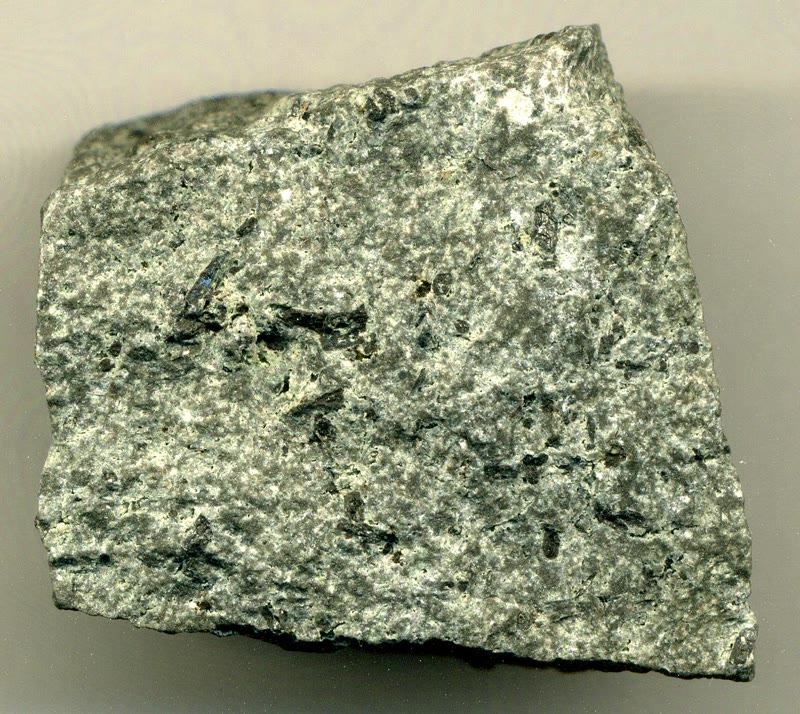
\includegraphics[height=4.4cm]{images/book2/g12-stjohn-andesite.jpg}\hspace{0.03\linewidth}%
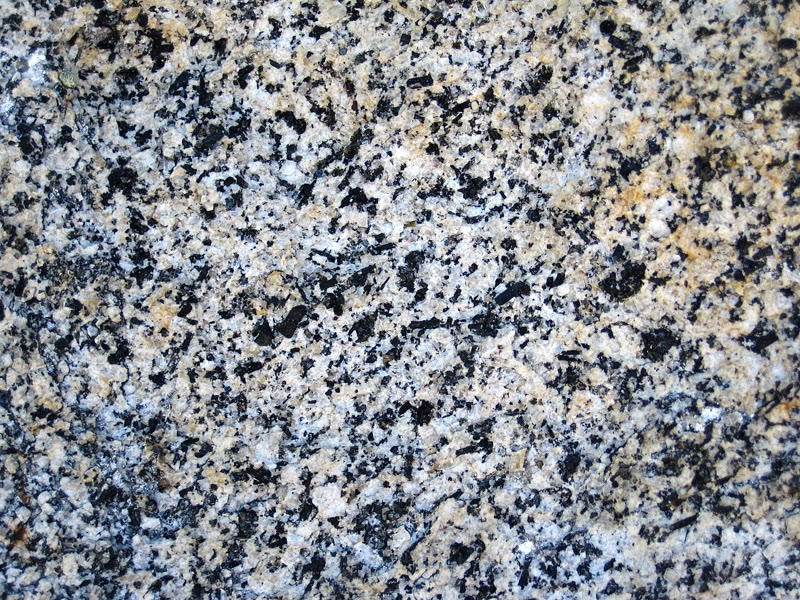
\includegraphics[height=4.4cm]{images/book2/g12-stjohn-granodiorite.jpg}

{\small À gauche~: une \omterm{def:g11:igneous-rocks:rock-names}{andésite}, \omterm{def:g11:igneous-rocks:volcanic-plutonic}{roche volcanique} à grain fin des arcs. À
droite~: une \omterm{def:g12:subduction-magmatism:granodiorite}{granodiorite} de la Sierra Nevada, avec du plagioclase blanc, du
quartz gris, et de la biotite et de la hornblende noires. Photographies
James St.~John (CC~BY~2.0).}
\end{omfigure}
% ledger: photo:g12-andesite, photo:g12-granodiorite

En moyenne, la \omterm{def:g12:continental-crust:continental-crust}{croûte continentale} supérieure contient environ
\qty{67}{\percent} de \ce{SiO2}~: elle est \omterm{def:g11:igneous-rocks:felsic-mafic}{felsique}, comme les granites que
les arcs fabriquent en grande quantité dans leurs \omterm{def:g12:subduction-magmatism:batholith}{batholites}.
% ledger: rg14:crust (upper crust SiO2 66.6 wt %), tulane:magma-types, tulane:intrusions

\begin{definition}[Batholite]\label{def:g12:subduction-magmatism:batholith}
Un \emph{batholite}\index{batholite} est une grande masse de \omterm{def:g11:igneous-rocks:volcanic-plutonic}{roche
plutonique} qui couvre plus de \qty{100}{km^2} là où l'érosion l'a mise à nu.
Il se forme là où de nombreux \omterm{def:g11:igneous-rocks:intrusion}{plutons}, mis en place les uns après les
autres, se rejoignent sous la surface.
\end{definition}
% ledger: earle:batholith, tulane:intrusions

L'un des plus grands du monde, le complexe \omterm{def:g11:igneous-rocks:volcanic-plutonic}{plutonique} de la Côte, longe la
côte pacifique depuis la région de Vancouver, dans l'ouest du Canada,
jusqu'au sud-est de l'Alaska. Le \omterm{def:g12:subduction-magmatism:batholith}{batholite} de la Sierra Nevada, en
Californie, s'est formé au-dessus d'une \omterm{def:g11:subduction-zones:subduction}{zone de subduction}~; la plupart de
ses granites de Yosemite ont cristallisé au Crétacé, il y a 105 à 85
millions d'années. Les roches qui les recouvraient ont été usées pendant des
millions d'années, et les \omterm{def:g11:igneous-rocks:intrusion}{plutons} refroidis en profondeur forment
aujourd'hui les montagnes.
% ledger: earle:batholith, nps:yosemite, photo:g12-sierra-nevada (St. John description), ics:base.Cretaceous

\begin{omfigure}
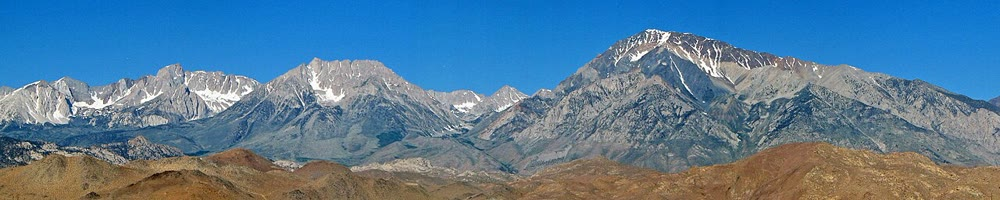
\includegraphics[width=0.94\linewidth]{images/book2/g12-stjohn-sierra-nevada-batholith.jpg}

{\small La Sierra Nevada, vue depuis l'est~: le granite et la \omterm{def:g12:subduction-magmatism:granodiorite}{granodiorite}
du \omterm{def:g12:subduction-magmatism:batholith}{batholite} de la Sierra Nevada, qui a cristallisé en profondeur au-dessus
d'une \omterm{def:g11:subduction-zones:subduction}{zone de subduction} au Crétacé. Photographie James St.~John
(CC~BY~2.0).}
\end{omfigure}
% ledger: photo:g12-sierra-nevada, nps:yosemite

\section{Comment les continents grandissent}

\begin{definition}[Croissance continentale]\label{def:g12:subduction-magmatism:continental-growth}
La \emph{croissance continentale}\index{croissance continentale} est
l'ajout de \omterm{def:g12:continental-crust:continental-crust}{croûte continentale} nouvelle, fabriquée à partir du manteau,
surtout par le magmatisme des arcs. La croissance nette des continents est
cet ajout moins la \omterm{def:g12:continental-crust:continental-crust}{croûte continentale} qui retourne dans le manteau.
\end{definition}
% ledger: sv09:growth, ss09:balance

C'est dans les arcs que se fabrique la roche légère des continents. Les
estimations du magma que les arcs ajoutent aujourd'hui sont d'environ
\qty{1.5}{km^3} par an aux arcs insulaires et de \qty{1.0}{km^3} par an aux
arcs continentaux~; en moyenne sur le long terme, environ \qty{2.7}{km^3}
par an. Mais les \omterm{def:g11:subduction-zones:subduction}{zones de subduction} renvoient aussi de la \omterm{def:g12:continental-crust:continental-crust}{croûte
continentale} dans le manteau~: des sédiments entraînés avec le \omterm{def:g11:subduction-zones:slab}{panneau
plongeant} et des morceaux de la plaque chevauchante arrachés par en
dessous, environ \qty{3.2}{km^3} par an. Les deux sont proches, et la
croissance nette des continents au cours des dernières centaines de
millions d'années a pu être nulle, voire négative.
% ledger: sv09:growth, ss09:balance

Les continents grandissent aussi par leurs bords d'une autre manière. La
\omterm{def:g12:continental-crust:continental-crust}{croûte continentale} est trop légère pour être subduite~: quand une plaque
amène un continent dans une fosse, les deux continents se soudent lors
d'une collision (\cref{ch:g12:mountain-building}). Chaque continent a un
cœur ancien, un \omterm{def:g12:continental-crust:craton}{craton}, entouré de ceintures de roches plus jeunes, les
\omterm{def:g12:continental-crust:root}{racines} déformées d'anciennes chaînes de montagnes, ajoutées les unes après
les autres à ses bords (\cref{ch:g12:continental-crust}).
% ledger: tulane:no-subduct (continental crust too buoyant to subduct), earle:collision, tulane:cratons

\section{Exercices}

\begin{exercise}[$\star$]\label{exo:g12:subduction-magmatism:1}
Donner le mot~: (a) une ligne de volcans parallèle à une fosse, sur la
plaque qui ne plonge pas~; (b) une fusion provoquée par l'ajout d'eau à une
roche~; (c) une \omterm{def:g11:igneous-rocks:volcanic-plutonic}{roche plutonique} contenant plus de plagioclase que de
feldspath potassique et plus de \qty{20}{\percent} de quartz~; (d) une
masse de \omterm{def:g11:igneous-rocks:volcanic-plutonic}{roche plutonique} de plus de \qty{100}{km^2}~; (e) l'ajout de
\omterm{def:g12:continental-crust:continental-crust}{croûte continentale} nouvelle fabriquée à partir du manteau.
\end{exercise}

\begin{exercise}[$\star$]\label{exo:g12:subduction-magmatism:2}
Le 18 mai 1980, la colonne de cendres du mont Saint Helens s'éleva à plus
de \qty{24}{km} en moins de 15 minutes. (1) Quelle fut sa vitesse moyenne
d'ascension minimale, en \unit{km/h} et en \unit{m/s}~? (2) La comparer à
la vitesse du souffle latéral, au moins \qty{480}{km/h}.
\end{exercise}

\begin{exercise}[$\star$]\label{exo:g12:subduction-magmatism:3}
Sur les 1214 volcans du catalogue actifs depuis la fin de la dernière
glaciation, 838 se dressent au-dessus d'une \omterm{def:g11:subduction-zones:subduction}{zone de subduction}. (1) Quel
pourcentage cela représente-t-il~? (2) De quel côté d'une fosse se trouvent
ces volcans~? (3) Pourquoi n'y en a-t-il aucun entre la fosse et le front
volcanique~?
\end{exercise}

\begin{exercise}[$\star$]\label{exo:g12:subduction-magmatism:4}
Une roche à gros grains contient \qty{25}{\percent} de quartz,
\qty{45}{\percent} de plagioclase, \qty{15}{\percent} de feldspath
potassique et \qty{15}{\percent} de biotite et de hornblende. (1) Quelle
fraction de son feldspath est du plagioclase~? (2) Est-ce une
\omterm{def:g12:subduction-magmatism:granodiorite}{granodiorite}~?
\end{exercise}

\begin{exercise}[$\star$]\label{exo:g12:subduction-magmatism:5}
Donner deux raisons pour lesquelles les volcans des arcs ont des éruptions
plus explosives que ceux des dorsales.
\end{exercise}

\begin{exercise}[$\star\star$]\label{exo:g12:subduction-magmatism:6}
(1) Un front volcanique se trouve à \qty{150}{km} de sa fosse, au-dessus
d'un \omterm{def:g11:subduction-zones:slab}{panneau plongeant} de pendage \ang{35}. À quelle profondeur se trouve
le \omterm{def:g11:subduction-zones:slab}{panneau} sous ce front~? (2) Comparer à la moyenne de \qty{105}{km}.
\end{exercise}

\begin{exercise}[$\star\star$]\label{exo:g12:subduction-magmatism:7}
Supposer que le \omterm{def:g11:subduction-zones:slab}{panneau plongeant} se trouve à \qty{105}{km} sous chaque
front volcanique. À quelle distance de la fosse se trouve le front quand le
\omterm{def:g11:subduction-zones:slab}{panneau} plonge de \ang{20}, et quand il plonge de \ang{45}~? Qu'est-ce que
cela indique sur l'endroit où chercher l'arc~?
\end{exercise}

\begin{exercise}[$\star\star$]\label{exo:g12:subduction-magmatism:8}
À \qty{100}{km}, la pression vaut environ \qty{3.16}{GPa}. (1) À l'aide de $T =
-5.104P^2 + 132.9P + 1120.7$ ($P$ en \unit{GPa}, $T$ en \unit{\celsius}),
calculer la température à laquelle la \omterm{def:g11:ocean-ridges:peridotite}{péridotite} sèche commence à y
fondre. (2) En présence d'eau, elle commence à fondre vers
\qty{1000}{\celsius}. De combien l'eau l'abaisse-t-elle~? (3) Le coin de
manteau y est, disons, à \qty{1300}{\celsius}. Fond-il à sec~? En présence
d'eau~?
\end{exercise}

\begin{exercise}[$\star\star$]\label{exo:g12:subduction-magmatism:9}
L'avalanche de débris du mont Saint Helens a déplacé environ
\qty{2.5}{km^3} de roches. Les arcs ajoutent environ \qty{2.7}{km^3} de
croûte nouvelle par an. (1) Combien de jours du magmatisme d'arc du monde
entier l'avalanche représente-t-elle~? (2) Pourquoi la comparaison ne
porte-t-elle que sur l'ordre de grandeur~?
\end{exercise}

\begin{exercise}[$\star\star$]\label{exo:g12:subduction-magmatism:10}
(1) Quelle quantité de croûte nouvelle les arcs ajoutent-ils en un million
d'années, à \qty{2.7}{km^3} par an~? (2) La \omterm{def:g12:continental-crust:continental-crust}{croûte continentale} contient
environ \qty{9e9}{km^3}. Combien de temps les arcs seuls mettraient-ils à
fabriquer ce volume, si rien n'en était perdu~? (3) Comparer à l'âge de la
Terre, 4.5~milliards d'années.
\end{exercise}

\begin{exercise}[$\star\star$]\label{exo:g12:subduction-magmatism:11}
(1) Dans la coupe du Japon, pourquoi laisse-t-on de côté de nombreux
séismes moins profonds que \qty{70}{km} pour ajuster le \omterm{def:g11:subduction-zones:slab}{panneau plongeant}~?
(2) Les séismes profonds se trouvent à \qty{116}{km} de profondeur à
\ang{140.5}~E et à \qty{80}{km} à \ang{141.5}~E, avec \qty{86.4}{km} par
degré. Calculer le pendage du \omterm{def:g11:subduction-zones:slab}{panneau}.
\end{exercise}

\begin{exercise}[$\star\star\star$]\label{exo:g12:subduction-magmatism:12}
Montrer que, pour un front situé à une distance $d$ de la fosse au-dessus
d'un \omterm{def:g11:subduction-zones:slab}{panneau} de pendage $\theta$, la distance mesurée le long du \omterm{def:g11:subduction-zones:slab}{panneau}
depuis la fosse jusqu'au point situé sous le front vaut $d/\cos\theta$.
Pour le Japon ($d = \qty{270}{km}$, $\theta = \ang{20}$), que vaut-elle~?
La plaque Pacifique se déplace vers le Japon à environ \qty{83}{mm} par
an~; en prenant cette vitesse tout le long du \omterm{def:g11:subduction-zones:slab}{panneau}, combien de temps un
morceau de fond marin met-il pour aller de la fosse jusque sous les
volcans~?
\end{exercise}
% ledger: usgs:tohoku (83 mm/yr)

\begin{exercise}[$\star\star\star$]\label{exo:g12:subduction-magmatism:13}
La chambre magmatique du mont Saint Helens est large d'environ \qty{1}{km}
et s'étend d'environ 6 à \qty{14}{km} de profondeur. (1) En l'assimilant à
un cylindre vertical, estimer son volume. (2) Le comparer aux
\qty{2.5}{km^3} de l'avalanche. (3) Calculer la \omterm{def:g12:metamorphic-rocks:lithostatic}{pression lithostatique} à
son sommet et à sa base ($\rho =
\qty{2830}{kg/m^3}$, $g = \qty{9.81}{m/s^2}$).
\end{exercise}

\begin{exercise}[$\star\star\star$]\label{exo:g12:subduction-magmatism:14}
Les arcs ajoutent environ \qty{2.7}{km^3} de croûte par an, et les \omterm{def:g11:subduction-zones:subduction}{zones de
subduction} en reprennent environ \qty{3.2}{km^3}. (1) Quelle est la
variation nette par million d'années~? (2) Sur 500 millions d'années,
quelle fraction d'une croûte de \qty{9e9}{km^3} cela représente-t-il~?
(3) Les auteurs jugent la croissance nette «~pratiquement nulle~». Pourquoi,
compte tenu de l'incertitude de chaque estimation~?
\end{exercise}

\begin{exercise}[$\star\star\star$]\label{exo:g12:subduction-magmatism:15}
Un \omterm{def:g12:subduction-magmatism:batholith}{batholite} met à nu \qty{20000}{km^2} de \omterm{def:g12:subduction-magmatism:granodiorite}{granodiorite} dont les \omterm{def:g11:igneous-rocks:intrusion}{plutons}
se sont solidifiés entre 5 et \qty{15}{km} de profondeur. (1) Estimer le
volume de magma qu'il représente, en lui donnant une épaisseur de
\qty{10}{km}. (2) À \qty{1}{km^3} par an, le rythme de tous les arcs
continentaux du monde réunis, combien de temps mettraient-ils à le
fabriquer~? Qu'est-ce que cela indique sur la durée de construction d'un
\omterm{def:g12:subduction-magmatism:batholith}{batholite}~?
(3) Quelle épaisseur de roches a dû être érodée au-dessus de lui avant
qu'on puisse le voir~?
\end{exercise}

\begin{problem}[{Problème du week-end --- sous les volcans du Japon}]
\label{pb:g12:subduction-magmatism:1}
% ledger: data:b2-usgs-ne-japan, data:gvp, data:pb2002, sa06:slab-depth, hirschmann:solidus, wang20:wet-solidus, earle:arc-water, data:prem
% values (arc_magmatism.py): Megata 139.725, Iwate 141.001, trench 144.12; bins 140.5/141/141.5: 116.4/98.15/80.35 km; P_100km 3.157, dry_T_100km 1489
Les volcans du nord-est du Japon situés entre \ang{37.5} et \ang{40.5}~N
s'étendent de \ang{139.7}~E (le Megata, le plus occidental) à
\ang{141.0}~E (l'Iwate, le plus oriental)~; la fosse du Japon se trouve à
\ang{144.1}~E. Le tableau donne la profondeur médiane des séismes plus
profonds que \qty{70}{km} dans trois bandes de longitude, de 1976 à 2025.
Prendre \qty{111.2}{km} pour un degré de latitude.

\begin{center}
\small
\begin{tabular}{|l|c|c|c|}
\hline
longitude (\unit{\degree}~E) & 140.5 & 141.0 & 141.5 \\ \hline
profondeur médiane (\unit{km}) & 116 & 98 & 80 \\ \hline
\end{tabular}
\end{center}

\medskip
\noindent\textbf{Partie I --- Le front volcanique.}
\begin{enumerate}
  \item Montrer qu'un degré de longitude vaut environ \qty{86.4}{km} à
        \ang{39}~N.
  \item À quelle distance de la fosse se trouve le front volcanique~?
  \item Quelle est la largeur de l'arc, de l'Iwate au Megata~?
  \item Sur quelle plaque les volcans se dressent-ils, et de quel côté de
        la fosse~?
  \item Pourquoi n'y a-t-il pas de volcans entre la fosse et l'Iwate~?
\end{enumerate}

\medskip
\noindent\textbf{Partie II --- La coupe des séismes.}
\begin{enumerate}[resume]
  \item De combien de kilomètres les profondeurs médianes changent-elles de
        \ang{140.5} à \ang{141.5}~E~?
  \item Sur quelle distance horizontale~?
  \item Calculer le pendage du \omterm{def:g11:subduction-zones:slab}{panneau plongeant}.
  \item Prolonger la droite depuis \ang{141.0}~E, \qty{98}{km}, jusqu'à la
        surface. Où l'atteint-elle, et à quelle distance de la fosse~?
  \item Proposer une raison pour laquelle le \omterm{def:g11:subduction-zones:slab}{panneau} est moins incliné près
        de la fosse que plus en profondeur.
\end{enumerate}

\medskip
\noindent\textbf{Partie III --- Le panneau plongeant sous les volcans.}
\begin{enumerate}[resume]
  \item Calculer $H = d\tan\theta$ avec la distance de la question~2 et un
        pendage de \ang{20}.
  \item La comparer à la profondeur médiane sous le front.
  \item Comparer les deux à l'intervalle mondial, de 72 à \qty{173}{km}, et
        à la moyenne, \qty{105}{km}.
  \item À quelle profondeur se trouve le \omterm{def:g11:subduction-zones:slab}{panneau} sous le Megata, d'après la
        droite de la question~9~?
  \item En prenant pour la croûte de l'arc une épaisseur d'environ
        \qty{35}{km}, le toit du \omterm{def:g11:subduction-zones:slab}{panneau} sous le front se trouve-t-il dans
        la croûte ou dans le manteau~? À quelle distance sous la base de la
        croûte~?
\end{enumerate}

\medskip
\noindent\textbf{Partie IV --- D'où vient l'eau.}
\begin{enumerate}[resume]
  \item Où l'eau du \omterm{def:g11:subduction-zones:slab}{panneau plongeant} est-elle entrée dans ses roches, et
        dans quel minéral une grande partie en est-elle retenue~?
  \item À \qty{100}{km}, la pression vaut environ \qty{3.16}{GPa}. Calculer
        le solidus sec à cette profondeur avec $T = -5.104P^2 + 132.9P + 1120.7$.
  \item En présence d'eau, le solidus se situe entre 950 et
        \qty{1000}{\celsius}. De combien l'eau l'abaisse-t-elle~?
  \item Pourquoi le \omterm{def:g11:subduction-zones:slab}{panneau} froid lui-même ne peut-il pas être la source du
        magma~?
  \item Conclure~: à quelle profondeur se trouve le \omterm{def:g11:subduction-zones:slab}{panneau plongeant} sous
        le front volcanique du nord-est du Japon~?
\end{enumerate}
\end{problem}
